\chapter{Marco Te\'orico}

Este capitulo est\'a basado en el libro \textit{Diffusion MRI} \cite{Basser2009}
y en las clases del Doctor Michael L. Lipton \cite{Lipton2014} disponibles online. 
En caso de querer profundizar en alg\'un tema, por favor referirse a estos. 

\section{Imagen por resonancia magnética}
Se denomina momento magn\'etico nuclear al momento magn\'etico que posee un 
\'atomo a causa del spin de sus protones y electrones. Cuando un prot\'on con 
momento magn\'etico $\vec{\mu}$ es puesto dentro de un campo magn\'etico, 
comenzara a preceder en torno a la direcci\'on de este \'ultimo con una 
frecuencia: 

$$ \omega = \vec{\mu} \times \vec{B} = g\vec{J} \times B $$

Denominada frecuencia de Larmor, donde $\omega$ es la velocidad angular; $g$ es
la relaci\'on giromagn\'etica del prot\'on; $\vec{J}$ es su momento angular y $B$
es la fuerza del campo. A su vez, la cantidad de energ\'ia del campo determinara
el \'angulo entre $\mu$ y el campo mientras sucede la precesi\'on
(Figura \ref{fig:nosignal}). Esto quiere decir que dado un $B$ suficientemente 
grande es posible hacer que la precesi\'on suceda en la direcci\'on transversal
del campo, lo cual permitir\'ia medir $|\mu|$ simplemente poniendo una bobina en
ese plano (Figura \ref{fig:signal}). Si uno realizara el experimento notar\'ia
que al apagar el campo, la se\~nal comienza a desvanecerse, esto es porque el
sistema comienza a perder energ\'ia provocando que el \'angulo entre $\mu$ y el
campo se achique. A este proceso se lo denomina relajaci\'on. \\

\begin{figure}[h!]

\begin{minipage}[b]{0.49\textwidth}
    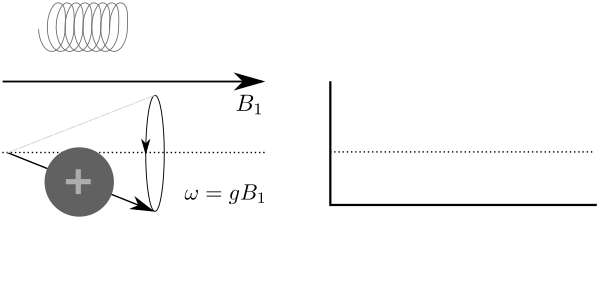
\includegraphics[width=\textwidth]{img/spin0.png}
    \caption{Spin sometido a un campo magn\'etico debil}
    \label{fig:nosignal}
\end{minipage} ~ %add desired spacing between images, e. g. ~, \quad, \qquad, \hfill etc. %(or a blank line to force the subfigure onto a new line) 
\hfill
\begin{minipage}[b]{0.49\textwidth}
    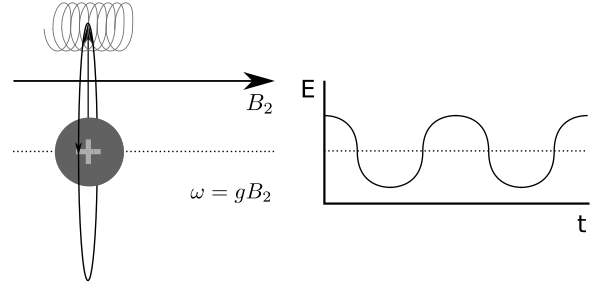
\includegraphics[width=\textwidth]{img/spin1.png}
    \caption{Resultado de aumentar el campo magn\'etico}
    \label{fig:signal}    
\end{minipage} ~ %add desired spacing between images, e. g. ~, \quad, \qquad, \hfill etc. %(or a blank line to force the subfigure onto a new line) 

\end{figure}

\vspace{0.1cm}
Vayamos ahora al plano m\'edico. El cuerpo est\'a compuesto por distintos 
tipos de tejidos, cada uno con su propia composici\'on qu\'imica, lo cual 
determina un momento magn\'etico distinto para cada uno de ellos, y por ende
un tiempo de relajaci\'on particular. Esto implica que al poner a un paciente
dentro de un campo magn\'etico, cada tejido comenzara a generar un momento 
en base a la poblaci\'on de protones que posea. Como ya fue dicho, una forma de
medir el tiempo de relajaci\'on de estos es utilizando un campo magn\'etico. 
El problema es que si uno intentara administrar energ\'ia al sistema simplemente
aumentando la fuerza del campo magn\'etico terminar\'ia da\~nando al paciente. 
Aqu\'i es donde se aprovecha la frecuencia de Larmor. Conociendo la composici\'on
qu\'imica de cada tejido es posible calcular su frecuencia angular. Luego, 
mediante el efecto de resonancia es posible transmitir energ\'ia al sistema
simplemente emitiendo ondas en esa misma frecuencia. \\

\begin{figure}[h!]
                                                                                                                        
\begin{minipage}[b]{0.49\textwidth}
    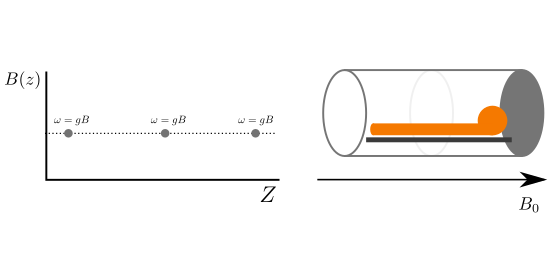
\includegraphics[width=\textwidth]{img/grad0.png}
    \caption{\small  Campo uniforme, todos los protones poseen la misma velocidad angular}
     \label{fig:unif}
\end{minipage} ~
\hfill
\begin{minipage}[b]{0.49\textwidth}
    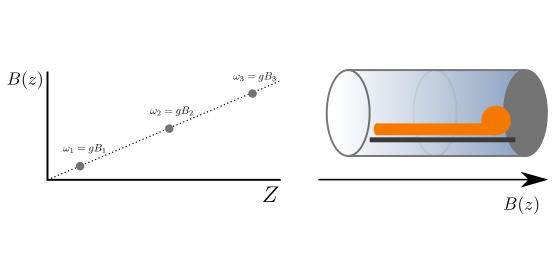
\includegraphics[width=\textwidth]{img/grad1.png}
    \caption{\small Campo gradiente, la velocidad angular de los protones var\'ia linealmente }
    \label{fig:grad}
\end{minipage} ~

\end{figure}  

\vspace{0.1cm}

Los resonadores magn\'eticos son dispositivos con la capacidad de generar 
campos y pulsos en diferentes frecuencias, en partocular todo resonador encendido
est\'a emitiendo constantemente un campo homog\'eneo $B_0$ (ver Figura \ref{fig:unif}). 
El problema entonces es: c\'omo obtener el tiempo de relajaci\'on 
de un punto particular del cuerpo. Para esto es posible utilizar campos 
gradientes. Un campo gradiente es un campo que var\'ia su potencia linealmente
a lo largo de una direcci\'on, provocando que todas los protones a lo 
largo de esa direcci\'on var\'ien su frecuencia angular de manera predecible. 
Aplicando un campo gradiente $G_z$ en la direcci\'on $z$ (ver Figura \ref{fig:grad})
sobre el paciente haremos que la velocidad en funci\'on de la posici\'on sea:
$\omega(z) = B_z(z) g$, esto nos asegurara que si aplicamos el pulso de RF a una
frecuencia de $B_z(z_o) g$, solo los protones que se encuentran en la posici\'on
$z=z_o$ comenzaran a resonar, por lo que estos ser\'an los \'unicos que generen un 
campo transversal. Cabe destacar que como no es posible generar un pulso con
exactamente la frecuencia deseada, tambi\'en resonaran los protones que se 
encuentren cerca, por lo que tendremos un intervalo $[z_o-\epsilon,z_o+\epsilon]$
resonando. A este proceso se lo denomina \textit{slice selection}. Podemos pensar 
el slice como una matriz de dos dimensiones sobre el eje $z$. Si ahora aplicamos
un campo gradiente $G_\psi$ en la direcci'on $y$, suceder\'a que todas las 
filas de nuestra matriz adquiriran diferentes velocidades angulares. Al apagar
$G_\psi$ todos los protones volveran a preceder respecto al campo $B_0$, pero
est\'a vez estaran desfasados por filas (ver Fig. \ref{fig:kspace}). Encendiendo
un tercer campo gradiente $G_\upsilon$ sobre la direcci\'on $x$ conseguiremos
que cada columna posea una frecuencia distinta y cada fila una fase distinta.
Repitiendo este procedimiento varias veces cambiando solo la intensidad de
$G_\psi$ podemos armar lo que se conoce como \textit{k-space}. El \textit{k-space}
es una imagen espacial temporal donde est\'an anotados los valores obtenidos para
cada potencia utilizada, en orden ascendente de potencia. El aplicar una
transformada de Fourier 3D a dicho espacio nos devolver\'a la imagen que
representa el contraste de cada tejido en el \textit{slice} seleccionado. \\

\begin{figure}[h!]
                                                                                                                        
\begin{minipage}[b]{\textwidth}
    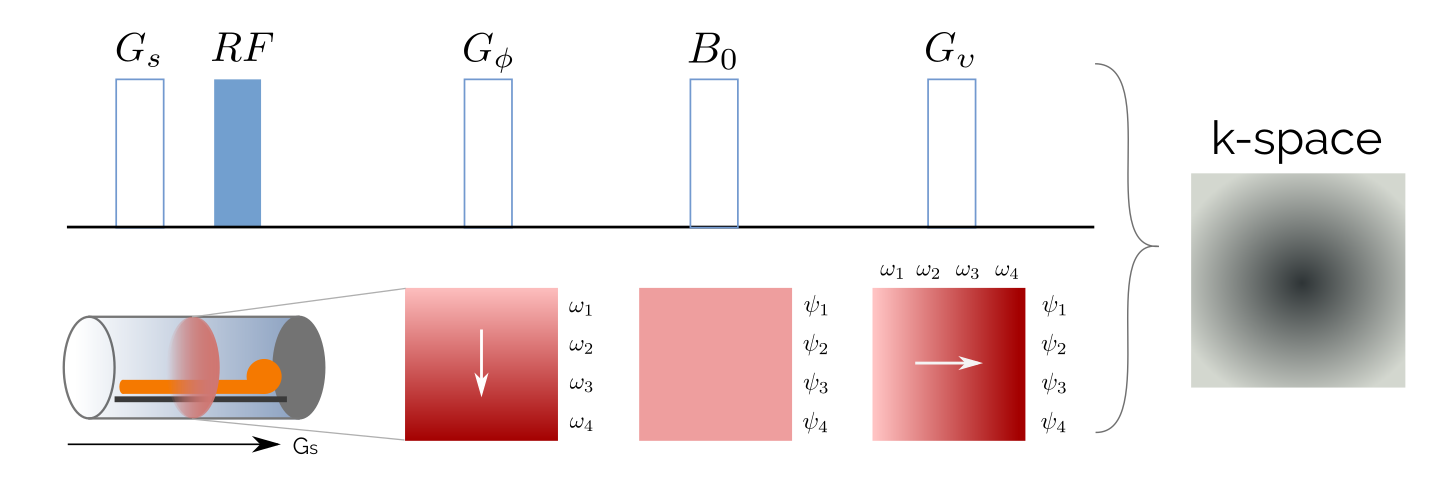
\includegraphics[width=\textwidth]{img/kspace.png}
    \caption{Resumen del proceso de adquisici\'on de im\'agenes en MRI}
    \label{fig:kspace}
\end{minipage} ~

\end{figure}  



\section{Resonancia Magn\'etica de Difusi\'on}

Las mol\'eculas dentro de un fluido en equilibrio no se encuentran est\'aticas,
sino que se mueven realizando un camino aleatorio. A este fen\'omeno se lo 
conoce con el nombre de difusi\'on.  \\

En 1946 Bloch \cite{Bloch1946} demostr\'o que la variaci\'on de la magnetizaci\'on
nuclear en el tiempo se puede expresar como:

$$ \frac{dM(t)}{dt} = g M(t) \times B(t) 
                      - \frac{M(t) \vec{x} + M(t)\vec{y}}{T_2}
                      - \frac{(M(t)-M(0))\vec{z}}{T1} $$

Donde $B$ es la intensidad del campo magn\'etico; T1 y T2 son tiempos de
relajaci\'on. Luego, en 1956, H.C. Torrey \cite{Torrey1956} agreg\'o a la
ecuaci\'on      los efectos de la difusi\'on:

$$ \frac{dM(t)}{dt} = g M(t) \times B(t) 
                      - \frac{M(t) \vec{x} + M(t)\vec{y}}{T_2}
                      - \frac{(M(t)-M(0))\vec{z}}{T1} 
                      + \nabla \cdot D \nabla M(t) $$

Donde a $D$ se lo conoce como el tensor de difusi\'on. Esta \'ultima relaci\'on
es conocida como la ecuaci\'on de Bloch-Torrey.\\

Imaginemos el siguiente experimento: luego de aplicar el pulso RF agregamos un
campo gradiente $G_1=G_d$ durante un tiempo $\delta$ peque\~no. Como ya explicamos,
esto generar\'a un desfase entre los spines de los protones. El aplicar $G_2=-G_d$
luego de $\Delta$ deber\'ia provocar que los spines se vuelvan a alinear. Sin
embargo, los protones que se encuentren en un fluido estar\'an sometidos al
efecto de la difusi\'on. Esto sucede, por ejemplo, en el interior de los
axones. Dependiendo del tiempo $\delta$ los protones se habr\'an movido cierta
distancia, provocando que el campo magn\'etico los alcance en distintas 
posiciones. Por ende su velocidad angular se ver\'a afectada de manera distinta 
a la esperada si no se hubieran movido. Esto nos indica que si hay difusi\'on
entonces habr\'a un desfase en esa poblaci\'on de neutrones (ver Figura 
\ref{fig:dmri}).\\

\begin{figure}
                                                                                                                        
\begin{minipage}[b]{\textwidth}
    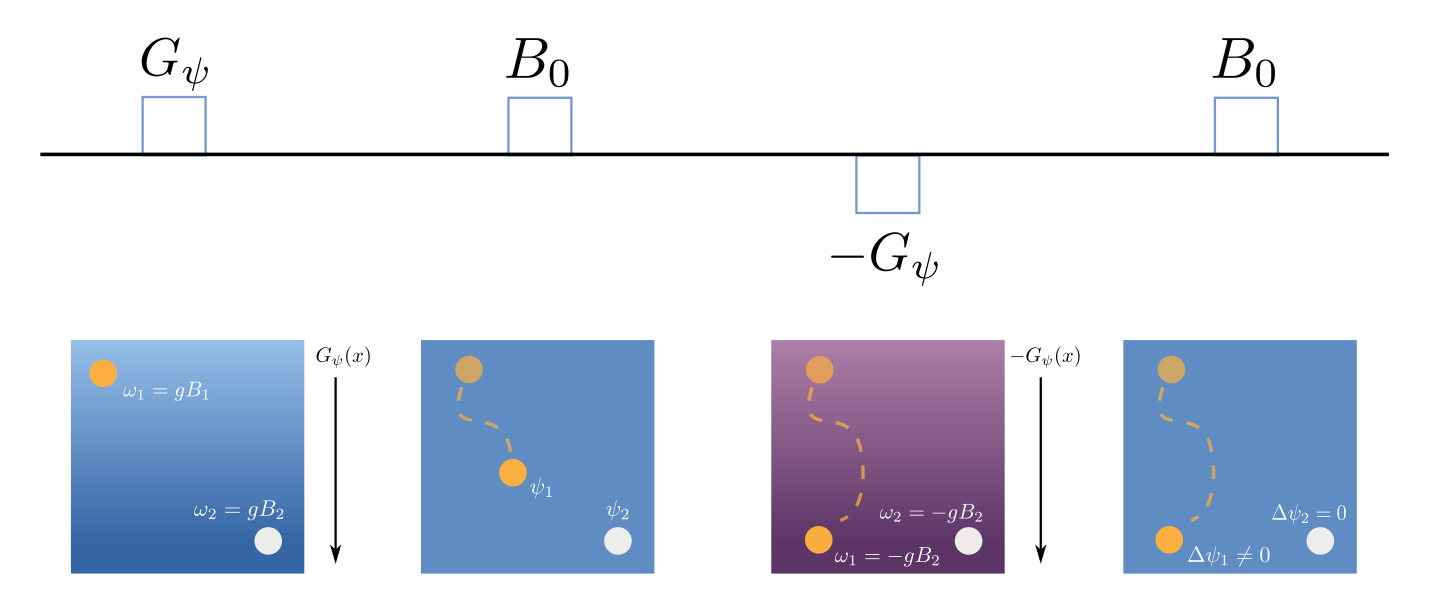
\includegraphics[width=\textwidth]{img/dmri.png}
    \caption{Modificar la secuencia permite medir la intensidad de difusi\'on}
    \label{fig:dmri}
\end{minipage} ~

\end{figure}  

Recordemos que la se\~nal medida en un resonador magn\'etico proviene del 
momento magn\'etico de los protones. Es importante entender que por limitaciones
f\'isicas de los dispositivos es imposible obtener la se\~nal producida por un
solo prot\'on. Lo que se mide es la resultante de los momentos magn\'eticos de 
todos los protones dentro de un espacio. Si todos los protones est\'an precediendo
a la misma velocidad sobre el mismo plano, entonces la resultante m\'axima se
obtiene cuando todos poseen la misma fase. Esto es, todos se encuentran en la
misma posici\'on al mismo tiempo, rotando juntos. Por ende, el desfase producto
de la difusi\'on se traducira en perdida de se\~nal.\\

\begin{wrapfigure}{r}{0.5\textwidth}
    \begin{center}
        \vspace{-1cm}
        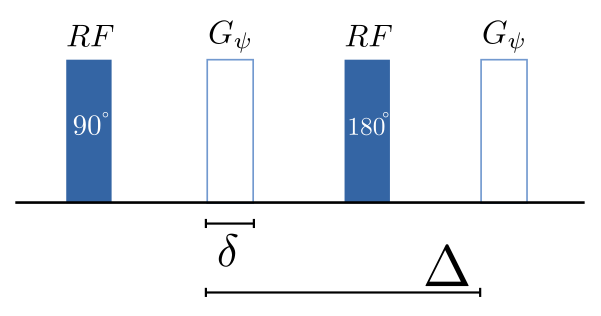
\includegraphics[width=0.4\textwidth]{img/fgp.png}
        \caption{Pulsed Gradient Spin Echo}
        \label{fig:fgp}
    \end{center}
\end{wrapfigure}  

En 1965 Stejskal y Tanner \cite{Stejskal1965} cren una secuencia denominada 
\textit{Pulsed Gradient Spin Echo}. En la misma utilizan dos pulsos de RF y 
un gradiente magn\'etico para generar un desfase entre los protones (ver Figura
\ref{fig:fgp}). Bajo estas condiciones la ecuaci\'on de Bloch-Torrey tiene
soluci\'on, y la atenuaci\'on de la se\~nal se puede expresar como:

\vspace{0.3cm}

$$ E(b) = \frac{S(b)}{S_0} = e^{-b D} $$
$$ b = -g^2 B^2 \delta^2 (\Delta^2 - \frac{\delta}{3}) $$ \\

\vspace{0.1cm}
 
Donde $E(b)$ es la atenuaci\'on de la se\~nal obtenida; $S_0$ es la se\~nal obtenida
sin utilizar gradientes de difusi\'on; $B$ es la intensidad del gradiente de
difusi\'on, $g$ es la relaci\'on giromagn\'etica;  $\delta$ es el tiempo que el
gradiente de difusi\'on est\'a encendido; $\Delta$ es el tiempo entre las 
activaciones del grediente y $D$ representa el coeficiente de difusi\'on.
El agrupar todos los par\'ametros del experimento dentro de $b$ fue propuesto por
Le Bihan \cite{LEBIHAN}.
La raz\'on por la cual se divide la se\~nal obtenida por $S_0$ es porque la
se\~nal en cada punto depende fuertemente de la densidad de protones que hay
en el mismo, si no ponderamos dicha densidad, es imposible comparar la intensidad
de difusi\'on en distintas regiones. \\

Basser et al. \cite{Basser1994} proponen medir la atenuaci\'on de se\~nal en
distintas direcciones y luego aproximar el coeficiente de difusi\'on con un 
tensor de segundo orden. Un tensor es una matriz multidimensional asociado a una
base, que posee una ley de transformaci\'on  para indicar  c\'omo cambian los 
componentes del tensor al cambiar de base. Esta t\'ecnica sienta las bases de lo
que se conoce como \textit{Diffusion Tensor Imaging} (DTI). En DTI el tensor 
mas utilizado representa un elipsoide en $R^3$. La matriz que lo representa
es  sim\'etrica, por ello es que se necesitan tomar al menos seis adquisiciones: 

$$
    D =
    \begin{pmatrix}
             D_{xx} & D_{xy} & D_{xz} \\
             D_{xy} & D_{yy} & D_{yz} \\
             D_{xz} & D_{yz} & D_{zz}    
    \end{pmatrix}
$$

\vspace{0.1cm}

El problema con utilizar este es que no permite representar correctamente
el cruce de fibras dentro de cada voxel dado que las caracteriza con un solo
elipsoide.\\

En 1991 Callaghan et al \cite{Callaghan1991} desarrollan el \textit{q-space analysis}.
Demuestran que sin asumir un modelo para la distribuci\'on de desplazamiento, 
pero tomando un $\delta$ chico, se deriva la siguiente relaci\'on entre la se\~nal
atenuada y una transformada de Fourier:

$$E(q,t) =  \frac{S(q,t)}{S_0} = \int_{R^2}{p(r,t)e^{-2\pi i q r} dr} $$
$$ q = \frac{g \delta B}{2\pi} $$

Donde $q$ es una medida que relaciona $B$ con $\delta$; $t$ es el tiempo durante
el cual se mide la se\~nal; $p(r,t)$ es la densidad de probabilidad de que una
poblaci\'on de part\'iculas se desplace en direcci\'on $r$ durante ese tiempo $t$.\\

Una de las principales ventajas de \textit{q-space} sobre DTI es que no asume
ning\'un modelo a priori, esto permite definir distintos tipos de modelos para
$p(r,t)$ que caracterizan mejor el cruce de fibras. \textit{Spherical Harmonics}
\cite{Tuch2004} o \textit{Constrained Spherical Deconvolution} \cite{Tournier2004}.
son ejemplos de ello. \\

